\documentclass[24pt, a0paper, portrait]{tikzposter}
\usepackage[utf8]{inputenc}

\title{Projekat iz predmeta Soft kompjuting - prebrojavanje ljudi}
\author{Bojan Popržen, SW16-2017}
\date{\today}
\institute{Fakultet tehničkih nauka, Univerzitet u Novom Sadu}

\usepackage{blindtext}
\usepackage{comment}

\usetheme{Board}

\begin{document}

\maketitle

\begin{columns}

	\column{0.5}

	\block{Uvod}{U ovom projektu rešavan je problem prebrojavanja ljudi u pokretu na određenoj podlozi. Ljudi se kreću po pravougaonom platou tamne boje, a kamera koja to beleži je postavljena iznad njih. Zadatak je da se prebroje ljudi koji makar jednom kroče na plato. Rešenje problema potrebno je evaluirati tako da je rešenje ono koje proizvede najmanju \textit{MAE}(eng. Mean Absolute Error) za 10 datih video klipova.
    \vspace{0.5cm}

    Rešenje ovog problema ima široku primenu u praksi. Moguće primene su: alarmiranje ukoliko je broj ljudi u određenom prostoru prevelik, merenje iskorišćenosti prostora i preusmeravanje ljudi ukoliko je on previše iskorišćen ili je pak nedovoljno iskorišćen, automatsko uključivanje sistema za nadzor itd.}

	\column{0.5}

	\block{Moduli rešenja}{Rešenje je podeljeno u tri modula: \textbf{modul za prepoznavanje podloge po kojoj se ljudi kreću}, \textbf{modul za prebrojavanje ljudi} i \textbf{modul za praćenje broja ljudi}. Ulaz modula za prepoznavanje podloge je jedan frejm video-klipa, a izlaz je isečak frejma koji prikazuje samo podlogu. Ulaz modula za prebrojavanje ljudi je isečak frejma koji prikazuje samo podlogu po kojoj se ljudi kreću, a izlaz je broj ljudi koji se trenutno nalaze na njoj. Ulaz modula za praćenje broja ljudi je trenutan broj ljudi, a izlaz je broj ljudi koji su makar jednom kročili na podlogu. Potrebno je napomenuti da se modul za prepozavanje podloge izvršava samo na početku prvog video-klipa, jer je kamera stacionarna.}

\end{columns}

\begin{columns}

	\column{0.5}
	\block{Modul za prepoznavanje podloge}{Modul treba da prepozna podlogu tako što će doneti pretpostavku da je ona pravougaona. Sledi pregled transformacija koje ovaj modul izvršava nad frejmom:  

	\vspace{0.15cm}

	\begin{center}
	 \textbf{Pretvaranje RGB slike u Grayscale sliku} - lakša obrada slike
	
	\end{center}
            \begin{tikzfigure}
                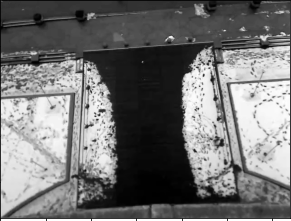
\includegraphics[width=0.15\textwidth]{assets/podloga-crno-belo.png}
            \end{tikzfigure}

	\begin{center}
	\textbf{Adaptivni threshold} - segmentacija slike, izdvajanje bitnog
	\end{center}
            \begin{tikzfigure}
                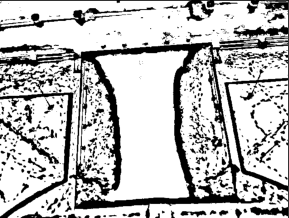
\includegraphics[width=0.15\textwidth]{assets/podloga-threshold.png}
            \end{tikzfigure}

	\begin{center}
	\textbf{Canny detekcija ivica} - detekcija važnih lokalnih oblika
	\end{center}
            \begin{tikzfigure}
                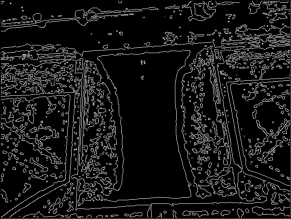
\includegraphics[width=0.15\textwidth]{assets/podloga-canny.png}
            \end{tikzfigure}

	\begin{center}
	\textbf{Hough detekcija linija} - detekcija graničnih linija podloge
	\end{center}
            \begin{tikzfigure}
                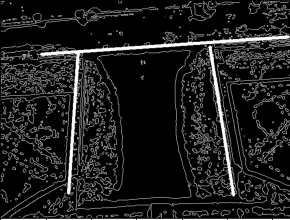
\includegraphics[width=0.15\textwidth]{assets/podloga-hough.png}
            \end{tikzfigure}

	\begin{center}
	\textbf{Pronalazak graničnih tačaka} - koordinate na osnovu koji se slika iseca
	\end{center}
            \begin{tikzfigure}
                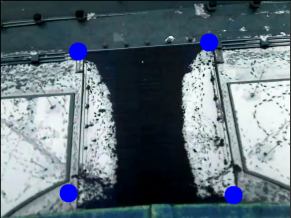
\includegraphics[width=0.15\textwidth]{assets/podloga-granicne-tacke.png}
            \end{tikzfigure}

	}
	\block{Evaluacija}{Evaluacija projekta}

	\column{0.5}
	\block{Modul za prebrojavanje ljudi}{Ovaj modul treba da prebroji ljude koji se nalaze na platou pretpostavljajući da su ljudi odeveni tako da odudaraju od same podloge. Modul izvršava sledeće transformacije nad ulaznom slikom:
	
	\vspace{0.15cm}

	\begin{center}
	 \textbf{Pretvaranje RGB slika u Grayscale slike} - obrađuju se slike trenutnog i prethodnog frejma
	
	\end{center}
            \begin{tikzfigure}
                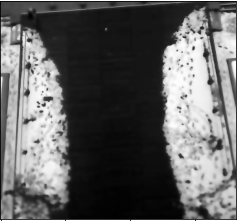
\includegraphics[width=0.15\textwidth]{assets/ljudi-prethodni-frejm.png}
	      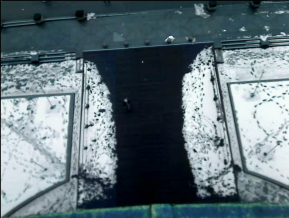
\includegraphics[width=0.15\textwidth]{assets/ljudi-trenutni-frejm.png}
            \end{tikzfigure}


	\begin{center}
	 \textbf{Razlika frejmova} - pošto se samo ljudi pomeraju
	
	\end{center}
            \begin{tikzfigure}
                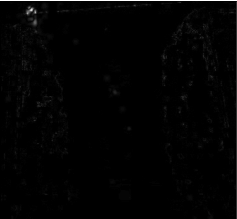
\includegraphics[width=0.15\textwidth]{assets/ljudi-razlika.png}
            \end{tikzfigure}

	\begin{center}
	 \textbf{Morfološko zatvaranje} - "finiranje" prostora između ljudi
	
	\end{center}
            \begin{tikzfigure}
                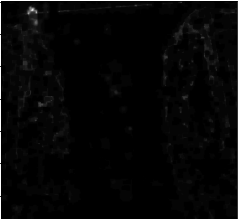
\includegraphics[width=0.15\textwidth]{assets/ljudi-morf-zatvaranje.png}
            \end{tikzfigure}

	\begin{center}
	 \textbf{Threshold} - segmentacija slike, izdvajanje bitnog
	
	\end{center}
            \begin{tikzfigure}
                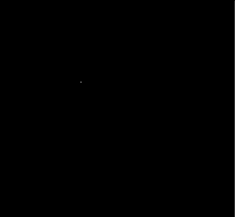
\includegraphics[width=0.15\textwidth]{assets/ljudi-threshold.png}
            \end{tikzfigure}

	\begin{center}
	 \textbf{Pronalazak kontura} - uočavanje objekata na slici i njihovo prebrojavanje
	
	\end{center}
            \begin{tikzfigure}
                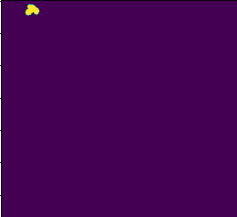
\includegraphics[width=0.15\textwidth]{assets/ljudi-konture.png}
            \end{tikzfigure}
}


\end{columns}



\end{document}